\chapter{Combustió}
 
\tableofcontents\newpage

\section{El motor de combustió interna}

Un motor de combustió interna (IC) és un conjunt d'elements mecànics que permeten obtenir energia mecànica a partir de l'estat tèrmic d'un fluid de treball generat en el seu propi interior mitjançant un procés de combustió.
 
Els motors de combustió interna, ja siguin alternatius o de reacció, són les principals fonts d'energia en el transport terrestre, marítim i aeri gràcies a la seva elevada potència específica. Aquests motors només competeixen amb els motors elèctrics en algunes aplicacions del transport ferroviari i, de manera creixent, en vehicles elèctrics purs o en configuració híbrida\cite{de_antonio_motores_2015}. 

En un motor de combusti\'o interna s'introdueix aire i combustible. En els motors d'encesa per espurna, la mescla d'aire i combustible es preparava antigament en el carburador i es condu\"ia al cilindre. Ara es realitza per mitj\`a d'injectors, cosa que permet un estalvi de combustible i un millor aprofitament d'aquest. En els motors d'encesa per compressi\'o (Diesel), la mescla es realitza directament dins del cilindre, on el combustible s'injecta despr\'es d'haver-hi introdu\"it i comprimit l'aire. Cada cilindre del motor t\'e una v\`alvula d'admissi\'o i una d'escapament, que s'obren i tanquen en el moment oport\'u per permetre l'entrada i sortida de gasos. Els motors típics tenen entre 3 i 12 cilindres, i la pot\`encia es pot augmentar afegint m\'es cilindres.

La paret de la cambra de combustió està formada per una camisa de ferro o alumini, i està inserida en un bloc de ferro o acer.

La mescla comprimida a la cambra de combusti\'o es transforma, per efecte de la combusti\'o, en vapor d'aigua (\ch{H2O}), di\`oxid de carboni (\ch{CO2}) i nitrogen (\ch{N2}). El nitrogen, un gas inert contingut a l'aire, no interv\'e en la combusti\'o. El vapor d'aigua produ\"it en la combusti\'o es mant\'e i es comporta com un gas permanent.

Entre els altres productes de la combusti\'o es troben altres gasos com: mon\`oxid de carboni (\ch{CO}), hidrogen (\ch{H2}), metà (\ch{CH4}) i oxigen (\ch{O2}), quan la combusti\'o \`es incompleta. La quantitat d'oxigen que participa en el proc\'es dep\`en directament de l'exc\'es d'aire introdu\"it respecte al necessari per a la combusti\'o.

En conseq\"u\`encia, el fluid de treball est\`a format inicialment per l'aire i el combustible i, despr\'es, pel conjunt de gasos produ\"its durant la combusti\'o. Com \`es evident, la seva composici\'o qu\'imica varia durant el cicle de treball.


\subsection{El motor de quatre temps}

    Un motor de quatre temps és aquell que necessita quatre recorreguts del pistó, dues voltes completes del cigonyal, per completar el seu cicle termodinàmic (veure animació a \url{https://www.grc.nasa.gov/www/k-12/airplane/engopt.html}).

    \newif\ifspark
\tikzset{tangent of circles/.style args={% https://tex.stackexchange.com/a/464143/194703
    at #1 and #2 with radii #3 and #4}{insert path={%
    let \p1=($(#2)-(#1)$),\n1={atan2(\y1,\x1)},\n2={veclen(\y1,\x1)*1pt/1cm},
    \n3={atan2(#4-#3,\n2)}
     in ($(#1)+(\n3+\n1+90:#3)$) coordinate(aux1) -- 
     ($(#2)+(\n3+\n1+90:#4)$) coordinate(aux2)}},
     pics/engine/.style={code={
  \tikzset{engine/.cd,#1}
  \draw[fill=gray!20] (0,0) -- (-0.8,-0.4) coordinate[pos=0.4] (p1)
  coordinate[pos=0.8] (p2) |- (-1,-3)[rounded corners=1mm] |- (-1.2,0) [sharp corners]
  -- (-1.2,0.7) coordinate[pos=0.2] (p3)
  coordinate[pos=0.8] (p4) -- (-0.9,0.85) -- (-0.6,0.7) -- (0,0.4) -- (0.6,0.7)
  -- (0.9,0.85)-- (1.2,0.7) -- (1.2,0)coordinate[pos=0.2] (p6)
  coordinate[pos=0.8] (p5) {[rounded corners=1mm] -- (1,0)}
  [sharp corners] -- (1,-3)
  -| (0.8,-0.4) -- cycle coordinate[pos=0.2] (p8)
  coordinate[pos=0.6] (p7);
  \draw[engine/left exhaust] (p1) to[bend right=18] (p4) -- (p3) to[bend left=18] (p2) -- cycle;
  \draw[engine/right exhaust] (p7) to[bend left=18] (p6) -- (p5) to[bend right=18] (p8) -- cycle;
  \draw[fill=gray!50] (0,-4) circle[radius=5mm];
  \pgfmathsetmacro{\pistonpos}{-4+0.4*sin(\pgfkeysvalueof{/tikz/engine/rod angle})
  +sqrt(1.5*1.5-pow(0.4*cos(\pgfkeysvalueof{/tikz/engine/rod angle}),2))}
  \path (0,-4) + (\pgfkeysvalueof{/tikz/engine/rod angle}:0.4) coordinate (p9)
   (0,\pistonpos) coordinate (p10);
  \draw[fill=gray!15] (p9) circle [radius=2mm] -- (p10) circle [radius=1mm];
  \path[tangent of circles={at p10 and p9 with radii 0.1 and 0.2}]
  (aux1) coordinate (aux3) (aux2) coordinate (aux4); 
  \path[tangent of circles={at p9 and p10 with radii 0.2 and 0.1}];
  \path[fill=gray!15] (aux1) -- (aux2) -- (aux3) -- (aux4);
  \draw  (aux1) -- (aux2)  (aux3) -- (aux4);
  \path[fill=gray!45] (p9) circle [radius=1.2mm];
  \begin{scope}
   \clip (-0.8,\pistonpos)   rectangle ++ (1.6,1);
   \draw[left color=gray!60,right color=gray!50,middle color=gray!10] (-0.8,\pistonpos) 
  rectangle ++ (2,1);
  \end{scope}
  \draw[left color=\pgfkeysvalueof{/tikz/engine/interior color}!80,
  right color=\pgfkeysvalueof{/tikz/engine/interior color}!50,
  middle color=white] 
  (-0.8,\pistonpos+1) --  (-0.8,-0.4)  -- (0,0)--  (0.8,-0.4) |- cycle;
  \draw[thin,fill=gray!30] (-0.42,-0.5) 
   ++ ({90+atan(1/2)}:0.25*\pgfkeysvalueof{/tikz/engine/left valve}) 
   -- ++ ({90+atan(1/2)}:1.9) -- ++ ({atan(1/2)}:0.1)
   -- ++ ({-90+atan(1/2)}:1.9) -- ++({atan(1/2)}:0.3)
   -- ++ ({-90+atan(1/2)}:0.1) -- ++({atan(1/2)+180}:0.7)
   -- ++ ({90+atan(1/2)}:0.1) -- cycle;
  \draw[thin,fill=gray!30] (0.42,-0.5) 
   ++ ({90-atan(1/2)}:0.25*\pgfkeysvalueof{/tikz/engine/right valve}) 
   -- ++ ({90-atan(1/2)}:1.9) -- ++ ({180-atan(1/2)}:0.1)
   -- ++ ({-90-atan(1/2)}:1.9) -- ++({180-atan(1/2)}:0.3)
   -- ++ ({-90-atan(1/2)}:0.1) -- ++({-atan(1/2)}:0.7)
   -- ++ ({90-atan(1/2)}:0.1) -- cycle;
  \draw[left color=gray!60,right color=gray!50,middle color=gray!10]
   (-0.1,-0.2) rectangle (0.1,1);   
  \ifspark
  \begin{scope}
   \clip (-1.8,-0.2) rectangle (1.8,\pistonpos+1.1);
   \path (0,-0.2) node[starburst, inner color=yellow, outer color=red,minimum size=1cm]{};
  \end{scope}
  \fi 
 }},engine/.cd,left valve/.initial=1,right valve/.initial=1,
 left exhaust/.style={fill=gray!50},
 right exhaust/.style={fill=gray!50},
 rod angle/.initial=30,interior color/.initial=white,
 spark/.is if=spark}
 \begin{center}
 \scalebox{0.8}{
\begin{tikzpicture}[] 
 \path (0,0) pic{engine={left valve=0,rod angle=-40,
  left exhaust/.style={fill=gray!10}}}
 (3.2,0) pic{engine={rod angle=-170,interior color=yellow}}
 (6.4,0) pic{engine={rod angle=105,interior color=orange,spark}}
 (9.6,0) pic{engine={rod angle=-80,interior color=red}}
 (12.8,0) pic{engine={right valve=0,rod angle=-170,interior color=purple,
    right exhaust/.style={fill=purple!30}}};
\end{tikzpicture}
 }
\end{center}

\begin{itemize}

\item{Primer pas o admissió}
En aquesta etapa, quan el pistó baixa des del Punt Mort superior (PMS o, en anglès, top dead center, TDC) al Punt Mort Inferior (PMI o, en anglès bottom dead center, BDC), permet que el nou combustible entri per la vàlvula d'injecció. Mentre s'obre aquesta vàlvula, la d'escapament es manté tancada.

\item{Segon pas o compressió}
Al final de l'execució anterior, el gas dins del cilindre es comprimeix per mitjà del moviment ascendent del pistó, de manera que la vàlvula d'injecció es tanca per la pressió.

\item{Tercer pas o explosió/expansió}
Després del temps de compressió, quan el pistó torna a la posició superior, s'obté la pressió màxima dins del cilindre. En el nostre cas, tenim un motor dièsel, per la qual cosa el combustible s'injecta polvoritzat i es crema per mitjà de la pressió i la temperatura dins del cilindre. Aleshores, l'expansió del gas fa que el pistó es mogui de nou cap avall; és en aquest moment quan es crea el treball de tot el procés. El treball d'expansió obtingut és aproximadament cinc vegades el treball de compressió necessari.

\item Quart pas o escapament
En aquest últim pas, el moviment superior del pistó fa que els gasos de combustió surtin a través de la vàlvula d'escapament. Quan el pistó està a la part superior, la vàlvula d'escapament es tanca i la injecció s'obre perquè tot el procés es torni a iniciar.
\end{itemize}

El cigonyal completa dues voltes (720 graus) per cada cicle de quatre temps. Així, el motor de quatre temps necessita dues voltes completes del cigonyal per completar el seu cicle termodinàmic.

Molts dels comportaments del motor es poden descriure mitjan\c{c}ant els conceptes de les lleis dels gasos. Per exemple, segons la llei de Boyle, quan augmenta el volum de la cambra de combusti\'o durant l'aspiraci\'o, la pressi\'o disminueix i permet que l'aire entri al cilindre. Durant la compressi\'o, el gas s'escalfa i augmenta la pressi\'o. L'expansi\'o dels gasos calents, descrita per la llei de Charles, \`es el mecanisme pel qual es captura l'energia de la combusti\'o i es converteix en energia mec\`anica per impulsar el vehicle\cite{bowers_understanding_2014}.

    \subsection{Fases del Cicle Otto ideal}

    La Figure \ref{fig:otto} mostra els processos termodinàmics que es donen en el cicle Otto\cite{morales_caracterizacion_nodate}:
\begin{enumerate}
    \item 0-1 Aspiraci\'o (proc\'es isoc\`oric): 
    La v\'alvula d'admissi\'o s'obre i s'aspira una c\`arrega d'aire i combustible a una pressi\'o te\`oricament igual a l'atmosf\`erica, provocant el descens del pist\'o. La v\'alvula d'escapament roman tancada. L'injector de fuel  genera un aerosol de combustible, en forma d'una fina boira de gotes minúscules, que es barreja amb l'aire aspirat.
    
    \item 1-2 Compressi\'o (proc\'es adiab\`atic):
    No existeix intercanvi de calor entre el gas i les parets del cilindre. La v\'alvula d'admissi\'o i la d'escapament estan tancades i el pist\'o comen\c{c}a a pujar, comprimint la mescla que es vaporitza.
    
    \item 2-3 Combusti\'o (proc\'es isoc\`oric):
    Ambdues v\'alvules romanen tancades. Quan el pist\'o arriba a la part superior del seu recorregut, el gas comprimit s'inflama per l'espurna de la bugia. La combusti\'o de tota la massa gasosa \`es instant\`ania, per la qual cosa el volum no variar\`a i la pressi\'o augmentar\`a r\`apidament. Això és degut a que la reacció genera molts més mols de gas que els inicials, i la temperatura augmenta enormement degut a la reacció química.
    
    \item 3-4 Expansi\'o (proc\'es adiab\`atic): 
    El gas inflamat empeny el pist\'o. Durant l'expansi\'o, no hi ha intercanvi de calor i, en augmentar el volum, la pressi\'o tamb\'e augmenta.
    
    \item 4-1 Escapament (proc\'es isoc\`oric)
    Quan el pist\'o es troba en l'extrem inferior del seu recorregut, la v\'alvula d'admissi\'o roman tancada i s'obre la d'escapament, disminuint r\`apidament la pressi\'o sense variar el volum interior. Despr\'es, mantenint la pressi\'o igual a l'atmosf\`erica, el volum disminueix.
\end{enumerate}
    
    
        \begin{figure}
            \centering
            \scalebox{0.8}{
    \begin{tikzpicture}[annotate/.style 2 args={postaction={decorate,decoration={markings,
        mark=at position 0 with {\node[circle,inner sep=1.5pt,draw,fill=white,#1]{};},
        mark=at position 0.5 with {\arrow[>=stealth,line width=1.5pt]{>};
        \node at (0,0.4) {#2};}}}}]
         \draw[stealth-stealth] (0,5) node[below left]{$p$} |- (5,0) node[below left]{$V$};
         \begin{scope}[thick]
          \draw[annotate={label=below right:1,alias=1}{$\dbar Q=0$}] plot[variable=\x,domain=4:1.5] (\x,{5/(\x+3)});
          \draw[annotate={label=below left:2,alias=2}{}] (1.5,5/4.5) -- (1.5,15/4.5);
          \draw[annotate={label=above left:3,alias=3}{$\dbar Q=0$}] plot[variable=\x,domain=1.5:4] (\x,{15/(\x+3)});
          \draw[annotate={label=above right:4,alias=4}{}] (4,15/7) -- (1);  
         \end{scope} 
         \path (2) -- (3) coordinate[pos=0.5] (23) (1) -- (4) coordinate[pos=0.5] (14);
         \draw[stealth-] ([xshift=-2mm]23) -- ++ (-1,0) node[midway,above]{$\Delta Q_h$};
         \draw[-stealth] ([xshift=2mm]14) -- ++ (1,0) node[midway,above]{$\Delta Q_c$};
         \draw[dashed] (1) -- (1|-0,0) node[below] {$V_1$};
         \draw[dashed] (2) -- (2|-0,0) node[below] {$V_2$};
        \end{tikzpicture}
        }
        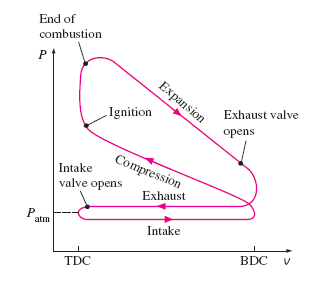
\includegraphics[scale=0.9]{../figures/Otto-real.png}
        \caption{La termodinàmica del cicle d'Otto. A l'esquerra, la situació ideal, on els processos d'expansió i compressió són adiabàtics, mentre que els de combustió i escapament són isocòrics. A la dreta, un esquema del cicle real.}
        \label{fig:otto}
    \end{figure}

    \subsection{Cicle Otto Real}

    El procés Otto real (Figura \ref{fig:otto}) s'allunya \href{http://tesla.us.es/wiki/index.php/Ciclo_Otto}{de forma significativa} de l'ideal. 



    \begin{enumerate}
        \item 0-1 Aspiraci\'o: 
        La pressi\'o del gas durant l'aspiraci\'o \'es inferior a la pressi\'o atmosf\`erica, per tant, el tancament de la v\'alvula d'admissi\'o es produeix despr\'es que el pist\'o arriba a l'extrem inferior de la seva carrera. Aix\`o prolonga el per\'iode d'admissi\'o i permet l'entrada de la m\`axima quantitat de mescla d'aire i combustible al cilindre.
        
        \item 1-2 Compressi\'o:
        El gas cedeix calor al cilindre, cosa que fa que es refredi i adquireixi menys pressi\'o.
        
        \item 2-3 Combusti\'o:
        La combusti\'o no \`es instant\`ania i el volum de la mescla varia mentre es propaga la inflamaci\'o. Per obtenir un m\`axim treball, \'es essencial triar el moment adequat per a l'encesa. La xispa ha de saltar abans que el pist\'o hagi finalitzat la carrera de compressi\'o, cosa que augmenta considerablement la pressi\'o assolida despr\'es de la combusti\'o i, per tant, el treball guanyat.
        
        \item 3-4 Expansi\'o: 
        L'augment de temperatura dins del cilindre durant la combusti\'o fa que, durant l'expansi\'o, els gasos cedeixin calor al cilindre i es refredin, resultant en una pressi\'o menor. Per tant, es tracta d'un procés no adiabàtic.
        
        \item 4-1 Escapament:
        En realitat, l'escapament no es produeix instant\`aniament. Els gasos encara tenen una pressi\'o superior a l'atmosf\`erica en aquest per\'iode. Per aix\`o, la v\'alvula d'escapament s'obre abans que el pist\'o arribi a l'extrem inferior del seu recorregut, permetent que la pressi\'o del gas disminueixi a mesura que el pist\'o acaba la seva carrera descendent. Quan el pist\'o realitza la seva carrera ascendent, troba davant seu gasos ja gaireb\'e totalment expandits. A m\'es, la v\'alvula d'admissi\'o s'obre abans que el pist\'o arribi a l'extrem superior del seu recorregut, generant una certa depressi\'o en el cilindre que afavoreix una aspiraci\'o m\'es en\`ergica.
    \end{enumerate}



\subsection{Cicle Diesel}

El motor Diesel \`es un motor de combusti\'o interna basat en el cicle Otto, per\`o amb la difer\`encia que el combustible s'injecta despr\'es de la compressi\'o de l'aire. 

Durant l'aspiraci\'o, entra nom\'es aire en el cilindre. En la compressi\'o, l'aire s'escalfa i, quan el pist\'o arriba al punt mort superior, s'injecta el di\`esel. Un motor diesel presenta uns factors de compressió molt més elevats que un motor Otto, i per tant, la temperatura de l'aire comprimit és molt més alta. Això permet que el dièsel s'encengui per la pressió i la temperatura de l'aire comprimit, sense necessitat d'una espurna. Finalment, l'escapament funciona de manera similar al motor d'encesa per espurna. 

Aquest motor permet una major efici\`encia t\'ermica i t\'e avantatges econ\`omics en diverses aplicacions. Tot i aix\`o, presenta dificultats t\`ecniques en sistemes d'injecci\'o i combusti\'o. Per garantir una combusti\'o neta i eficient, el proc\'es es realitza en mi\lgem isegons. Els motors Diesel usen ratios combustible/aire molt més baixos, amb la qual cosa la combustió és més completa.





    \section{Reaccions de combustió}

    Per definici\'o, una reacci\'o de combusti\'o \`es qualsevol reacci\'o entre un material i un oxidant [t\'ipicament \ch{O2 (g)}] que allibera energia en forma de calor. Les reaccions qu\'imiques alteren els tipus d'enlla\c{c}os i les posicions relatives dels \`atoms dins de les mol\'ecules. Els materials inicials s'anomenen reactius, i els materials finals despr\'es de la reordenaci\'o s'anomenen productes. En una reacci\'o de combusti\'o, el material inicial no oxidant s'anomena combustible i pot ser una varietat de compostos qu\'imics\cite{bowers_understanding_2014}.

Normalment, la combusti\'o es presenta en qu\'imica general i org\`anica com la reacci\'o dels combustibles hidrocarbonats amb l'oxigen per produir di\`oxid de carboni i aigua:
\begin{equation}
\ch{CH4 + 2 O2 -> CO2 + 2 H2O}
\end{equation}

No obstant aix\`o, els combustibles org\`anics contenen m\'es elements que nom\'es carboni i hidrogen, i produeixen altres gasos a banda del di\`oxid de carboni i l'aigua. Els motors de combusti\'o interna tamb\'e generen combustibles hidrocarbonats no cremats i els anomenats NOx t\'ermics, gasos amb la f\'ormula \ch{NO_x} que es formen quan el nitrogen atmosf\`eric es torna molt calent i reacciona amb l'oxigen atmosf\`eric. Aquests gasos contribueixen a les emissions dels motors i es redueixen mitjan\c{c}ant tecnologies d'emissions que es tractaran més endavant.


\subsection{Desti\lgem ació del petroli}

La majoria de motors de combustió interna de gasolina i dièsel estan dissenyats per utilitzar fraccions específiques d'hidrocarburs obtingudes del petroli cru. El petroli és una barreja complexa de compostos orgànics provinents de la descomposició de microorganismes marins enterrats. Només els components més lleugers i volàtils són adequats com a combustible per a vehicles\cite{bowers_understanding_2014}.

Aquests components se separen del petroli mitjançant desti\lgem ació, un procés on el líquid s'escalfa fins a bullir, i els vapors es refreden i es condensen en un recipient. En la desti\lgem ació industrial, això es fa en una torre de desti\lgem ació, un cilindre metà\lgem ic on els diferents components del petroli es condensen a diferents alçades segons el seu punt d'ebullició. Els compostos més lleugers surten per la part superior com a vapor, mentre que els més pesats es condensen més avall (Figura \ref{fig:torredestillacio}).

\begin{figure}
    \centering
    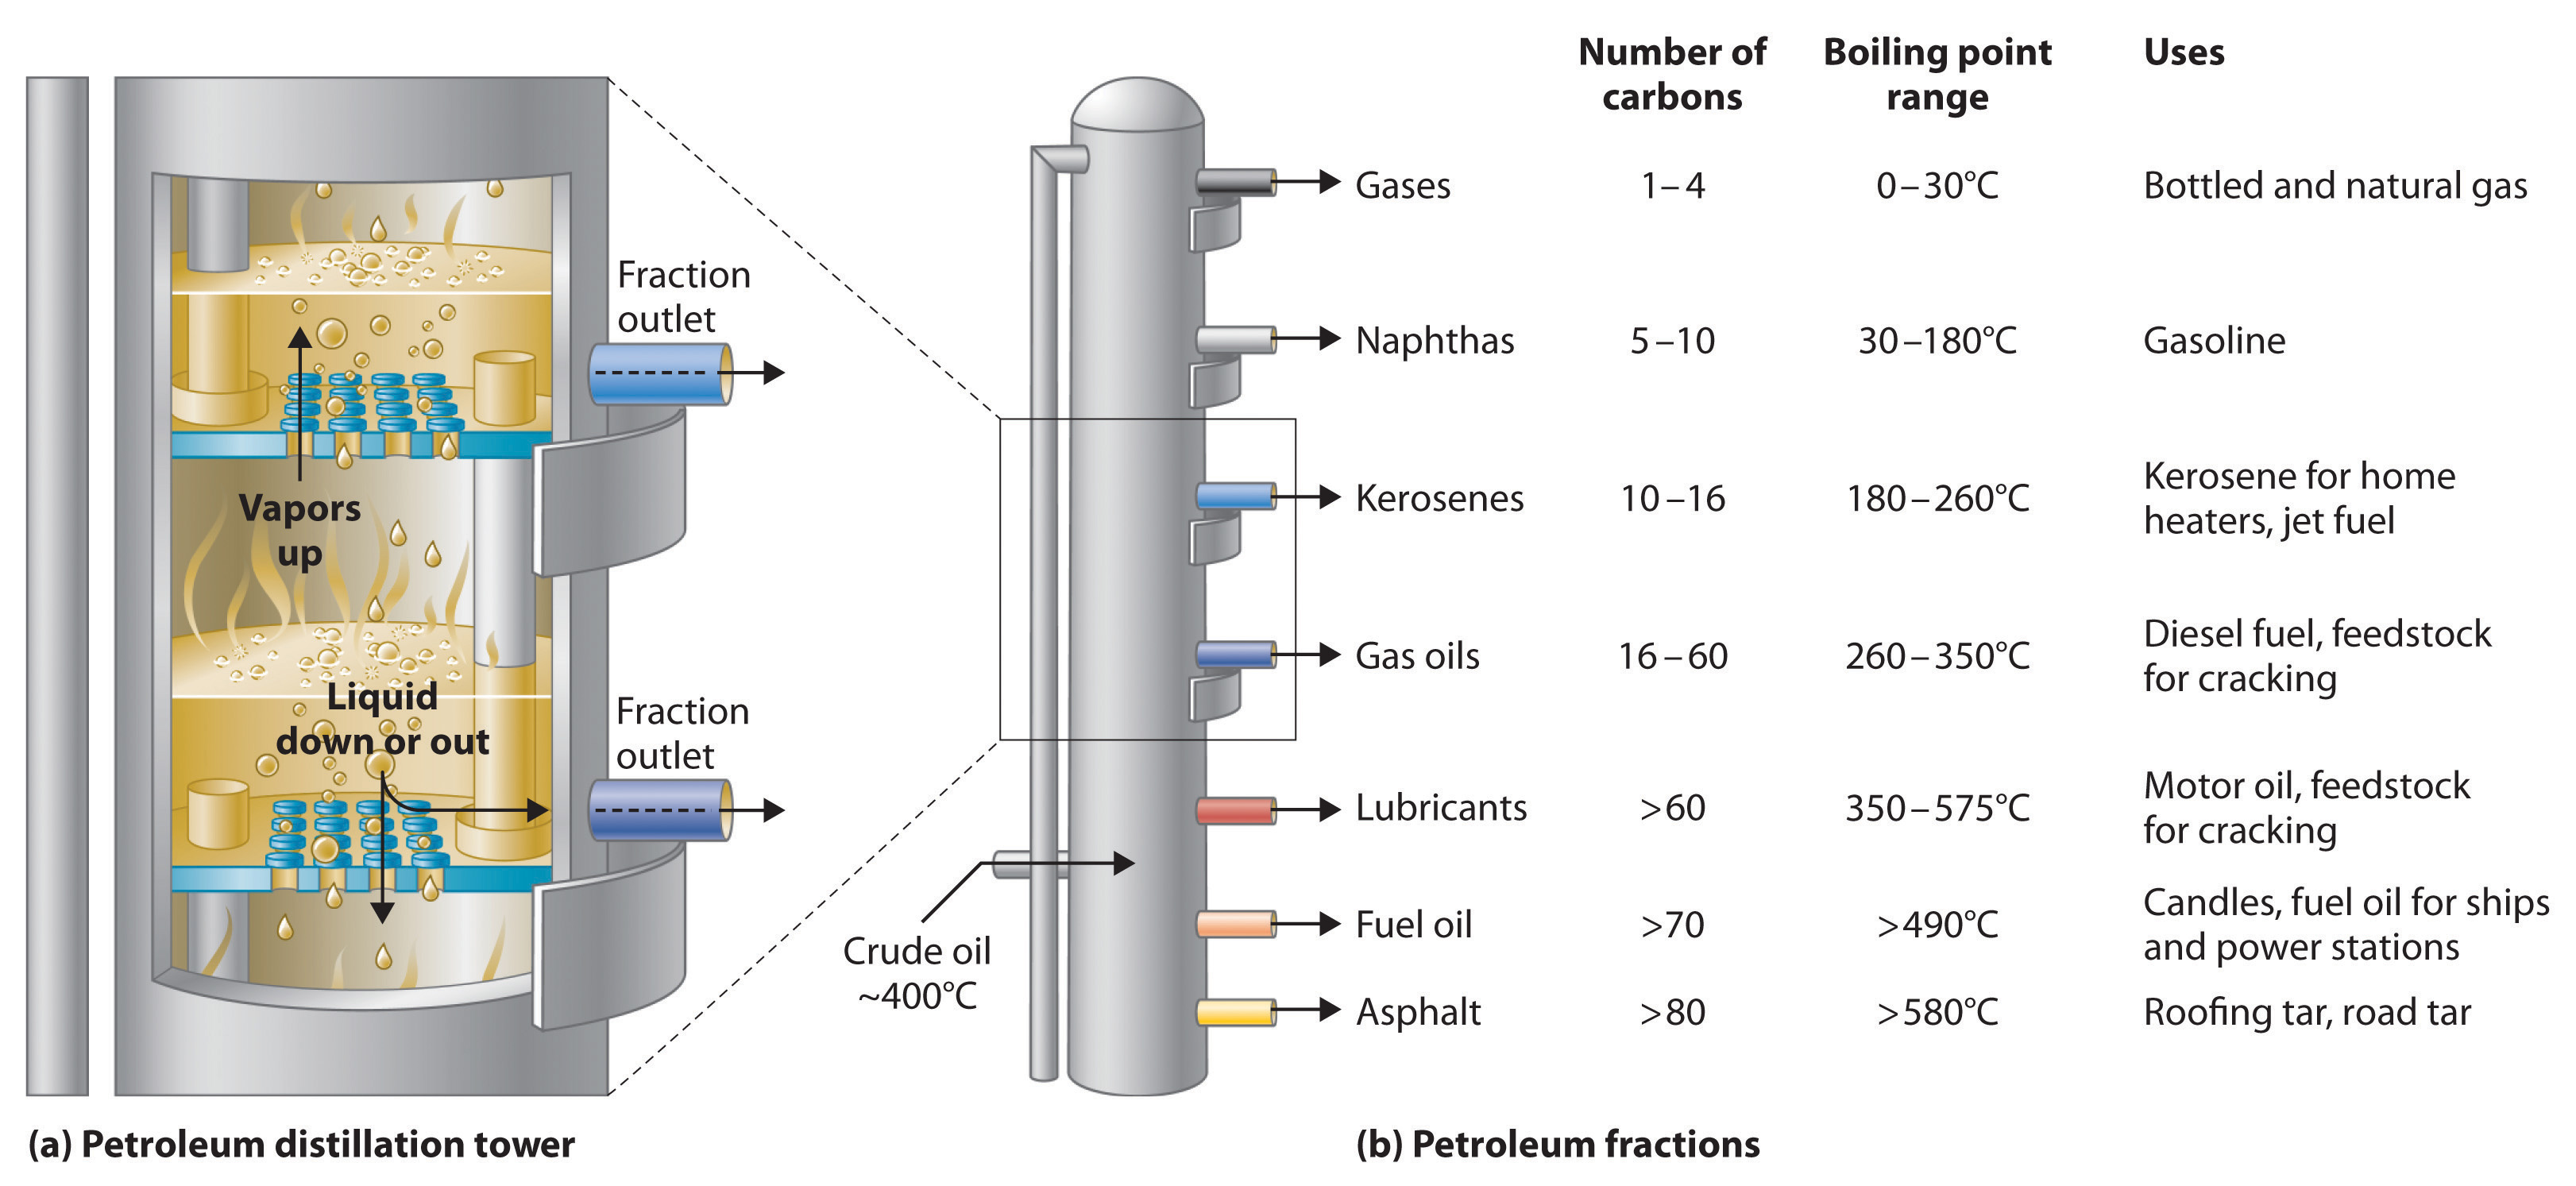
\includegraphics[width=\textwidth]{TorreDestillacio.jpg}
    \caption{Desti\lgem ació fraccionada del petroli\cite{noauthor_38_2015}.}
    \label{fig:torredestillacio}
\end{figure}


El dièsel es desti\lgem a entre 200°C i 350°C i conté hidrocarburs amb entre 8 i 21 àtoms de carboni. La gasolina, més volàtil, conté alcans lieals (parafines), alcans cíclics (naftalens) i alquens (olefines) de 4 a 12 carbonis i es desti\lgem a a temperatures més baixes, pel fet de ser més volàtil. Tant la gasolina com el dièsel inclouen additius químics per millorar la seva estabilitat i resistència a la compressió. Aquests additius solen ser substàncies orgàniques contenir nitrogen, fòsfor i oxigen, i també compostos aromàtics (anells de carboni amb enllaços híbrids).

Per simplificar, l'anàlisi de la combustió es centrarà en la gasolina i un dels seus principals components, l'octà, tot i que el mateix principi s'aplica a altres combustibles.

\subsection{L'índex d'octà}

    Què significa el número d'octà de la benzina o per què alguns cotxes necessiten gasolina premium? El número d'octà mesura la resistència del combustible a la ignició espontània quan es comprimeix.

    L'octà, o n-octà, és un hidrocarbur de la família dels alquans amb fórmula molecular \ch{C8H18}. És un líquid incolor, inodor i inflamable. És un component important de la gasolina, ja que té una estructura lineal que li permet tenir una alta resistència a la detonació. Això fa que sigui un combustible ideal per a motors d'alta compressió.

En un motor de combustió interna, el combustible ha de cremar quan s'encén la bugia. Si la compressió fa que es detoni abans d'horaes poden danyar components com vàlvules i pistons. Això es coneix com a picat de biela o preignició.

El número d'octà es determina en un laboratori, cremant el combustible en un motor amb ràtio de compressió variable fins que es detecta el picat. A partir d'això, es compara amb una barreja de \href{https://www.ebi.ac.uk/chebi/searchId.do?printerFriendlyView=true&chebiId=62805&structureView=applet}{isooctà} i heptà amb la mateixa resistència a la detonació. El número d'octà indica el percentatge d'isooctà en aquesta barreja equivalent. Per exemple, un combustible amb un número d'octà de 90 té la mateixa resistència a la preignició que una barreja del 90\% d'isooctà i 10\% d'heptà (veure Taula \ref{tab:octa}).

És important saber que aquest número no indica la quantitat real d'octà en la benzina. Hi ha altres compostos amb més resistència a la detonació que poden donar valors superiors a 100. En resum, com més alta sigui la ràtio de compressió del motor, més alt ha de ser el número d'octà per evitar problemes de preignició.  
\
\begin{table}[h!]
    \centering
    \caption{Taula de compostos amb les seves fórmules condensades i índex d'octà (Adaptada de \cite{noauthor_38_2015}). }
    \renewcommand{\arraystretch}{1.5}
    \scriptsize
    \begin{tabular}{p{1cm}cc|p{1cm}cc}
        \toprule
        \textbf{Nom} & \textbf{Fórmula } & \textbf{Índex} & \textbf{Nom} & \textbf{Fórmula } & \textbf{Índex} \\
        \midrule
        n-heptà & \ch{CH3-(CH2)5-CH3} & 0 &
        o-xilè & \chemfig{[:-30]**6(--(-CH3)-(-CH3)--(-[,,,,,draw=none])-)} & 107 \\
        n-hexà & \ch{CH3-(CH2)4-CH3} & 25 & 
        etanol & \ch{CH3CH2OH} & 108 \\
        n-pentà & \ch{CH3-(CH2)3-CH3} & 62 &
        t-butil alcohol & \ch{(CH3)3COH} & 113 \\
        isooctà & \ch{(CH3)3CCH2CH(CH3)2} & 100 &
        p-xilè & \chemfig{[:-30]**6((-CH3)---(-CH3)---)} & 116 \\
        benzè & \chemfig{[:-30]**6(------)} & 106 &
        metil terc-butil èter & \ch{H3COC(CH3)3} & 116 \\
        metanol & \ch{CH3OH} & 107 &
        toluè & \chemfig{[:-60]*6(-=-=(-CH3)-=)} & 118 \\
        \bottomrule
    \end{tabular}
    \normalsize
    \label{tab:octa}
\end{table}


Molts compostos actuals tenen un índex d'octà superior a 100, cosa que els fa millors combustibles que l'isooctà pur. A més, s'han desenvolupat agents anticolp, també anomenats potenciadors d'octà. Durant molts anys, un dels més utilitzats va ser el tetraetilplom \ch{(C2H5)4Pb}, que a una concentració d'aproximadament \qty{11.36}{\gram\per\litre} augmentava l'índex d'octà en 10-15 punts. No obstant això, des de 1975, els compostos de plom han estat progressivament eliminats com a additius de la gasolina a causa de la seva elevada toxicitat.

Per substituir-los, es van desenvolupar altres potenciadors com el metil terc-butil èter (MTBE), que té un índex d'octà elevat i causa poca corrosió al motor i al sistema de combustible. Tanmateix, les fuites de gasolina amb MTBE des de dipòsits subterranis han contaminat aigües subterrànies en algunes zones, fet que ha portat a restriccions o prohibicions del seu ús. Com a alternativa, s'està promovent l'ús d'etanol, que es pot obtenir de fonts renovables com el blat de moro, la canya de sucre o les gramínies.

\section{Termodinàmica de la combustió}

Les reaccions químiques poden ser, a nivell del calor que intercanvien amb l'entorn:
\begin{description}
\item[exotèrmiques] si desprenen calor i, per tant, l'energia dels productes és més baixa que la dels reactius; o bé
\item[endotèrmiques] si l'absorbeixen i els productes acaben tenint més energia que els reactius.
\end{description}

En moltes ocasions mirem d'obtenir treball a partir de la calor produïda en una reacció, com succeix, per exemple, en un procés de combustió o en les reaccions electroquímiques que fan funcionar motors de combustió o elèctrics. La calor generada per la combustió d'una quantitat de combustible s'anomena calor de combustió, i es mesura en \si{\joule\per\mole}. Aquesta quantitat varia segons el combustible i la seva composició.

La termodinàmica estudia les relacions entre energia, calor i treball.
En aquest capítol treballarem al voltant de la termoquímica, la termodinàmica associada a les reaccions químiques, no només a la combustió

\begin{mybox}[title={Sistemes, estats i funcions d'estat}]
    Anomenem \emph{sistema} a aquella part de l'\emph{univers} que volem tractar en algun càlcul o experiment. 
Per exemple, un sistema pot ser un cilindre en un motor de combustió o bé una bateria elèctrica.
\begin{center}
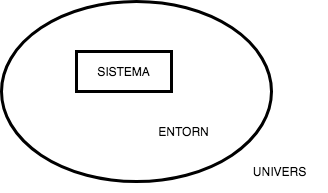
\includegraphics[scale=0.5]{SistEntornUnivers.png}
\end{center}
 
L'\textit{estat del sistema} es caracteritza  per unes determinades \textit{variables d'estat} ($P$, $V$, $T$, $E$, $H$,...), magnituds físiques macroscòpiques mesurables. La termodinàmica estudia els \textit{estats d'equilibri} dels sistemes, en els quals les variables d'estat són idèntiques en totes les seves parts i invariables en el temps:
\begin{enumerate}
\item En els \textit{canvis d'estat} d'un sistema, les variables d'estat només depenen de l'estat inicial i final, i no del camí utilitzat. Així, per exemple, el treball $w$ no és funció d'estat, mentre que l'energia $E$ sí que ho és.
\item En fixar els valors d'algunes d'elles, una equació d'estat determina automàticament el valor de les altres. Així, per exemple, en un gas ideal, si coneixem $P$, $V$ i $T$, podem determinar $E$, $H$, $S$, etc.
\end{enumerate}

Els canvis d'estat poden ser 
\begin{description}
\item[reversibles] quan les funcions d'estat varian de manera infinitessimal, mantenint el sistema constantment en l'equilibri (l'expansió d'un gas contra una pressió que difereix només $dP$ de la pressió interna, per exemple);
\item[irreversibles] en qualsevol altre situació (un procés de combustió, l'expansió d'un gas contra el buit, etc).
\end{description}
\end{mybox}

\subsection{Treball}

El treball realitzat per una força en desplaçar un cos entre dues posicions es calcula segons:
\[
w=\int_{x_1}^{x_2} \mathbf{F} \cdot \mathbf{dx}
\]
Tenint en compte que $P=\frac{F}{A}$, és fàcil veure que, en el cas d'un pistó que exerceixi una pressió externa sobre un gas 
\begin{center}
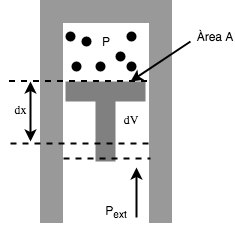
\includegraphics[scale=0.6]{pisto_dw.png}
\end{center}
tenim
\[
dw=-F_{ext}dx = -P_{ext} A dx = -P_{ext} dV
\]
i, per tant,
\[
w=-\int_{V_1}^{V_2} P_{ext} dV
\]
\begin{EXMP}[Treball en una expansió isobàrica]

Considerem un gas ideal que s'expandeix isobàricament (a pressió constant) des d'un volum inicial $V_1$ fins a un volum final $V_2$. El treball realitzat pel gas durant aquesta expansió es pot calcular com:

\[
w = -P_{\text{ext}} \Delta V = -P_{\text{ext}} (V_2 - V_1)
\]

On $P_{\text{ext}}$ és la pressió externa constant. Si la pressió està en \si{\pascal} i el volum en \si{\meter\cubed}, el treball es mesura en \si{\joule}.

Per exemple, si un gas s'expandeix des de \qty{1}{\meter\cubed} fins a \qty{2}{\meter\cubed} a una pressió constant de \qty{100}{\kilo\pascal}, el treball realitzat pel gas és:

\[
w = -\qty{100}{\kilo\pascal} \times (\qty{2}{\meter\cubed} - \qty{1}{\meter\cubed}) = -\qty{100}{\kilo\pascal} \times \qty{1}{\meter\cubed} = -\qty{100}{\kilo\joule}
\]

El signe negatiu indica que el treball és realitzat pel sistema (el gas) sobre l'entorn.
\end{EXMP}



\subsection{Calor}

La calor $q$ és una magnitud macroscòpica que representa l'efecte d'infinitud de treballs microscòpics deguts als moviments de les partícules d'un sistema.
Com el treball, no és una funció d'estat, ja que depèn del camí que utilitzem per transferir-lo.
La calor es medeix en calories o Joules.\marginnote{Definim com caloria la quantitat de calor necessària per escalfar 1 gr d'aigua \qty{1}{\degC}. Per tant, la capacitat calorífica de l'aigua és $C_p=\qty{1}{\cal\per\gram\per\degC}$. En realitat, això només és cert per a una temperatura donada, ja que la capacitat calorífica depèn lleugerament de la temperatura de partida. En el cas de l'aigua, la caloria es defineix per al pas de 14.5\unit{\degC} a 15.5\unit{\degC}. La quantitat de treball necessària per produir aquesta calor es va determinar per Mayer y Joule el s. XIX com \qty{1}{\cal}=\qty{4.1860}{\joule}. En química usem més sovint les Capacitats calorífiques molars, $C_m$,  que indiquen la quantitat de calor necessària per escalfar un mol d'una substància 1\unit{\degC}.}

La quantitat de calor necessària per incrementar la temperatura un determinat valor d'\qty{1}{\mole} de substància és
\[
q=nC_m\Delta T
\]
Si aquesta expressió la usem per explicar un procés infinitessimal obtenim
\[
C_m=\frac{1}{n}\frac{dq}{dT}
\]
I com que la capacitat calorífica es pot obtenir a $V=\text{cnt}$ o a $P=\text{cnt}$, podem calcular
\[
q_v=\int_{T_1}^{T_2} n C_{v,m} dT
\]
i
\[
q_p=\int_{T_1}^{T_2} n C_{p,m} dT
\]

\begin{EXMP}[Calor en un procés isocòric]

Considerem ara un gas ideal que s'escalfa isocòricament (a volum constant) des d'una temperatura inicial $T_1$ fins a una temperatura final $T_2$. La calor transferida al gas durant aquest procés es pot calcular com:

\[
q_v = n C_{v,m} \Delta T = n C_{v,m} (T_2 - T_1)
\]

On $n$ és el nombre de mols de gas, $C_{v,m}$ és la capacitat calorífica molar a volum constant, i $\Delta T$ és el canvi de temperatura. Si la capacitat calorífica està en \si{\joule\per\mole\per\kelvin} i la temperatura en \si{\kelvin}, la calor es mesura en \si{\joule}.
\end{EXMP}

\subsection{Primera llei de la termodinàmica}

La primera llei de la termodinàmica estableix que l'energia no es pot crear ni destruir, sinó que es pot transformar d'una forma a una altra. Això es pot expressar com:
\begin{equation}
    \Delta U = q + w
\end{equation}
on $\Delta U$ és la variació d'{\bf energia interna}, $q$ és la calor transferida al sistema i $w$ és el treball realitzat sobre el sistema. $U$ és una {\bf funció d'estat}, ja que el seu increment $\Delta U$ depèn només de l'estat inicial i final, no del camí seguit per arribar-hi. És per això que l'escrivim en majúscules, a diferència de la calor i el treball, que són funcions de camí.

Imaginem una reacció que es dona a pressió constant. En aquest cas, la calor transferida al sistema és la calor de combustió, i el treball realitzat és el treball de compressió. Així, la primera llei de la termodinàmica es pot reescriure com:
\begin{equation}
    \Delta U = q - P \Delta V
\end{equation}
on $P$ és la pressió i $\Delta V$ és el canvi de volum.
En forma integral, si la pressió no fos constant, això es pot expressar com:
\begin{equation}
    \Delta U = q - \int_{V_1}^{V_2} P \diff V
\end{equation}

Si la reacció estudiada fos a volum constant, és a dir, en un recipient tancat, el treball de compressió seria zero i la primera llei es reduiria a:
\begin{equation}
    \Delta U = q_v
\end{equation}

Per tant, per mesurar la calor de combustió d'un combustible, es pot utilitzar un calorímetre a volum constant, on tota l'energia alliberada per la reacció es converteix en calor. Les reaccions que desprenen calor s'anomenen \textbf{exotèrmiques}, mentre que les que l'absorbeixen s'anomenen \textbf{endotèrmiques}. Si el sistema absorbeix calor, la variació d'energia interna serà positiva, i si la despren, serà negativa.

Normalment, però, les reaccions químiques succeeixen a pressió constant, i per tant, la calor de combustió es mesura a pressió constant. Això es pot fer amb un calorímetre a pressió constant, on la calor de combustió es converteix en treball de compressió. En aquest cas, ens convé més usar una altra funció d'estat, l'{\bf entalpia}, que es defineix com:
\begin{equation}
    H = U + PV
\end{equation}
i la calor de combustió es pot expressar com:
\begin{equation}
    \Delta H = \Delta U + \Delta (PV) = q+ w + \Delta (PV) \end{equation}
    cal notar que a pressió constant, $w = -P \Delta V$, i $\Delta (PV)=P\Delta V$. Per tant,
    \begin{equation}
    \Delta H = q_p
\end{equation}

Novament, per a un procés exotèrmic a pressió constant, la variació d'entalpia serà negativa, ja que el sistema allibera calor. Això és el que succeeix en una reacció de combustió.

Cal notar que $\Delta H$ i $\Delta U$ són funcions d'estat, però no són iguals, ja que $H$ inclou el treball de compressió. No obstant això, en processos en solució, el treball de compressió és negligible i $\Delta U \approx \Delta H$.

\subsection{Increment d'entalpia estàndard}

L'increment d'entalpia estàndard d'una reacció, $\Delta H^\circ$, és la variació d'entalpia que es produeix quan els reactius en els seus estats estàndard es converteixen en productes en els seus estats estàndard. Els estats estàndard es defineixen a una pressió d'1 bar i una temperatura específica, generalment 298.15 K (25°C). Aquesta magnitud és molt útil per calcular la calor alliberada o absorbida en una reacció química, ja que permet comparar diferents reaccions en condicions similars. Per exemple, l'increment d'entalpia estàndard de la combustió del metà és:
\begin{equation}
\ch{CH4(g) + 2 O2(g) -> CO2(g) + 2 H2O(l)} \quad \Delta H^\circ = -890.3 \, \si{\kilo\joule\per\mole}
\end{equation} 

Aquesta equació indica que la combustió d'un mol de metà allibera 890.3 kJ d'energia en forma de calor. Els valors d'increment d'entalpia estàndard per a moltes reaccions es poden trobar en taules termodinàmiques\cite{lide_crc_2005} (algunes estàn recollides en la \href{https://biocomputing-teaching.github.io/WebQuimicaAutomocio/pdf/TaulaUnitats.pdf}{taula de paràmetres termodinàmics} del curs).

\subsection{Llei de Hess}

La llei de Hess estableix que el canvi d'entalpia d'una reacció química és independent del camí seguit per arribar als productes finals, depenent només dels estats inicial i final. Això permet calcular l'entalpia de reaccions complexes a partir de reaccions més senzilles. Per exemple, considerem la combustió del propà (\ch{C3H8}):
\begin{equation}
\ch{C3H8(g) + 5 O2(g) -> 3 CO2(g) + 4 H2O(l)}
\end{equation}

Podem descompondre aquesta reacció en passos més simples basats en les entalpies de formació (veure \href{https://biocomputing-teaching.github.io/WebQuimicaAutomocio/pdf/TaulaUnitats.pdf}{taula de paràmetres termodinàmics}):
\begin{align}
\ch{C3H8(g) -> 3 C(s) + 4 H2(g)} & \quad \Delta H_1^\circ = 104.7 \, \si{\kilo\joule\per\mole} \\
\ch{C(s) + O2(g) -> CO2(g)} & \quad \Delta H_2^\circ = -393.5 \, \si{\kilo\joule\per\mole} \\
\ch{H2(g) + 1/2 O2(g) -> H2O(l)} & \quad \Delta H_3^\circ = -285.8 \, \si{\kilo\joule\per\mole}
\end{align}

L'entalpia total de la reacció de combustió es pot calcular, aleshores, sumant les entalpies dels passos individuals:
\begin{equation}
\Delta H^\circ = \Delta H_1^\circ + 3 \Delta H_2^\circ + 4 \Delta H_3^\circ
\end{equation}

Substituint els valors:
\begin{equation*}
\Delta H^\circ = 104.7 + 3(-393.5) + 4(-285.8) = 104.7 - 1180.5 - 1143.2 = -2219 \, \si{\kilo\joule\per\mole}
\end{equation*}

Així, la llei de Hess ens permet determinar l'entalpia de reaccions complexes utilitzant dades d'entalpia de reaccions més simples.

L'{\bf entalpia estàndard de formació}, $\Delta H_f^\circ$ és la variació d'entalpia que es produeix quan un mol d'una substància es forma a partir dels seus elements en els seus estats estàndard. L'entalpia d'una reacció es pot calcular a partir de les entalpies de formació estàndard dels reactius i productes utilitzant la següent fórmula:

\begin{equation}
\Delta H^\circ_{\text{reacció}} = \sum \Delta H^\circ_f (\text{productes}) - \sum \Delta H^\circ_f (\text{reactius})
\end{equation}

La Figura \ref{Fig:combustioGlucosa}, per exemple, mostra el cicle termodinàmic que ens permet calcular l'entalpia de combustió de la glucosa a partir d'entalpies de formació tabulades.

\begin{figure}[htbp]
    \centering
        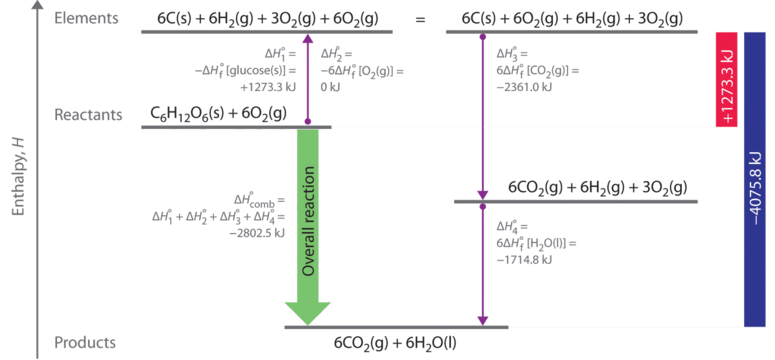
\includegraphics[width=0.9\textwidth]{Hess1.png}
    \caption{Cicle termodinàmic de la combustió de la glucosa.
    La fletxa verda etiquetada \(\Delta H^\circ_{\text{comb}}\) representa la reacció de combustió. Alternativament, podríem primer convertir els reactius en els elements mitjançant la inversió de les equacions que defineixen les seves entalpies estàndard de formació (fletxa ascendent, etiquetada com \(\Delta H^\circ_1\) i \(\Delta H^\circ_2\)).      
    A continuació, podríem convertir els elements en els productes mitjançant les equacions que defineixen les seves entalpies estàndard de formació (fletxes descendents, etiquetades com \(\Delta H^\circ_3\) i \(\Delta H^\circ_4\)).  
        Com que l'entalpia és una funció d'estat, es compleix que:  
    $\Delta H^\circ_{\text{comb}} = \Delta H^\circ_1 + \Delta H^\circ_2 + \Delta H^\circ_3 + \Delta H^\circ_4$. Adaptat de \cite{noauthor_78_2015}}
    \label{Fig:combustioGlucosa}
\end{figure} 

\subsection{Capacitat calorífica}   

Com hem vist més amunt, la capacitat calorífica es pot expressar com:
\begin{equation}
    C = \frac{q}{\Delta T}
\end{equation}

La capacitat calorífica a pressió constant es denota com $C_p$ i a volum constant com $C_v$. La diferència entre ambdues és el treball de compressió, i es pot expressar, en el cas dels gasos, com:
\begin{equation}
    C_p - C_v = R
\end{equation}

En el cas de líquids i sòlids, les dues capacitats calorífiques són pràcticament iguals, ja que el treball de compressió és negligible. En el cas dels gasos, la capacitat calorífica a pressió constant és lleugerament més gran que a volum constant, ja que el treball de compressió és positiu. 

\begin{table}[h!]
    \caption{Capacitats calorífiques (\si{\cal\per\mole\per\kelvin}) de diverses substàncies a 298 K i a pressió constant\cite{mahan_quimica_1997}.}
    \centering
    \renewcommand{\arraystretch}{1.5}
    \begin{tabular}{ccc|ccc}
        \toprule
        Substància & Fórmula & $C_p$  & Substància & Fórmula & $C_p$  \\
        \midrule
        Monòxid de carboni & \ch{CO} & 6.97 & Metà & \ch{CH4} & 8.53 \\
        Oxigen & \ch{O2} & 7.05 & Nitrogen & \ch{N2} & 6.97 \\
        Diòxid de carboni & \ch{CO2} & 8.96 & Hidrogen & \ch{H2} & 6.88 \\
        Aigua (vapor) & \ch{H2O(g)} & 8.02 & Etanol & \ch{C2H5OH} & 26.9 \\
        Propà & \ch{C3H8} & 17.6 & Butà & \ch{C4H10} & 23.5 \\
        \bottomrule
    \end{tabular}

    \label{tab:capacitats_calorifiques}
\end{table} 

\begin{mybox}[title=Relació entre la capacitat calorífica a pressió constant i a volum constant] 
Per deduir aquesta relació, considerem la primera llei de la termodinàmica:
\[
    \Delta U = q - P \Delta V
\]

A volum constant, el treball de compressió és zero ($\Delta V = 0$), i per tant. 
\[
    \Delta U = q_v = C_v \Delta T
\]

A pressió constant, la calor afegida al sistema es descompon en l'increment d'energia interna i el treball de compressió. 
\[
    q_p = \Delta U + P \Delta V = C_p \Delta T
\]

Utilitzant l'equació d'estat dels gasos ideals, $P \Delta V = nR \Delta T$, i per a $n = 1$ podem escriure:
\[
    C_p \Delta T = C_v \Delta T + R \Delta T
\]
 i, per tant:
\[
    C_p - C_v = R
\]

\end{mybox}

La capacitat calorífica es pot expressar en forma diferencial com:

\begin{equation}
    C_v = \left( \frac{\partial U}{\partial T} \right)_V = \left( \frac{\partial q_v}{\partial T} \right)_V
\end{equation}

\begin{equation}
    C_p = \left( \frac{\partial H}{\partial T} \right)_P = \left( \frac{\partial q_p}{\partial T} \right)_P
\end{equation}

\subsection{Dependència de l'entalpia amb la temperatura}

L'entalpia d'una substància depèn de la temperatura. Imaginem que volem calcular l'entalpia d'una reacció a una temperatura $T_2$ a partir de l'entalpia a una temperatura $T_1$. Com que l'entalpia és una funció d'estat, podem calcular la variació d'entalpia entre $T_1$ i $T_2$ seguint aquest camí:

\begin{center}
    \schemestart
      \ch{a A + b B}
      \arrow{->[\state{H}^{}_1$(T_2)$]}[,1.5]
      \ch{c C + d D}
      \arrow{<-[\state{H}^{prod}$(T_2\to T_1)$]}[-90,2]
      \ch{c C + d D}
      \arrow{<-[\state{H}^{}_2$(T_1)$]}[180,1.5]
      \ch{a A + b B}  
      \arrow(@c4--@c1){->[\state{H}^{react}$(T_1\to T_2)$]}
    \schemestop
    \end{center}

Podem obtenir la variació d'entalpia com (recordem que la variació d'entalpia és precisament la variació de calor a pressió constant):

\begin{equation}
    \Delta H_2 = \Delta H_1 + \int_{T_1}^{T_2} C_p(\text{productes})\, dT - \int_{T_1}^{T_2} C_p(\text{reactius})\, dT.
\end{equation}

Si definim la diferència de calor específica:
\begin{equation}
    \Delta C_p = C_p(\text{productes}) - C_p(\text{reactius}),
\end{equation}
les integrals es poden combinar en:
\begin{equation}
    \Delta H_2 = \Delta H_1 + \int_{T_1}^{T_2} \Delta C_p dT.
\end{equation}

En el cas que $\Delta C_p$ sigui constant, la integral es resol com:
\begin{equation}
    \Delta H_2 = \Delta H_1 + \Delta C_p (T_2 - T_1).
    \label{eq:entalpia_temperatura}
\end{equation}

\begin{EXMP}[Càlcul de l'entalpia a una altra temperatura]
    Per exemple, donada la reacció:
    \begin{center}
    \ch{CO + $\frac{1}{2}$ O2 -> CO2}
    \end{center}
amb $\Delta H_{298} = \qty{-67.640}{\cal}$, calculem $\Delta H^\circ$ a \qty{398}{\kelvin}. De la Taula \ref{tab:capacitats_calorifiques}, tenim:   
\begin{align*}
    C_p(\ch{CO}) &= \qty{6.97}{\cal\per\mole\per\kelvin},\\
    C_p(\ch{O2}) &= \qty{7.05}{\cal\per\mole\per\kelvin},\\
    C_p(\ch{CO2}) &= \qty{8.96}{\cal\per\mole\per\kelvin}
\end{align*}
Substituïm a la fórmula \ref{eq:entalpia_temperatura}:
\begin{align*}
    \Delta C_p &= 8.96 - 6.97 - \frac{7.05}{2} = \qty{-1.53}{\cal\per\mole\per\kelvin},\\
    \Delta H_{398} &= \Delta H_{298} - \Delta C_p (\qty{398}{\kelvin} - \qty{298}{\kelvin})\\
    &= \qty{-67.640}{\cal} - (\qty{-1.53}{\cal\per\mole\per\kelvin} \times \qty{100}{\kelvin})\\
    &= \qty{-67.793}{\cal} = \qty{-283.6}{\kilo\joule\per\mole}.    
\end{align*}
\end{EXMP}

\section{Turbocompressors}

En qualsevol reacció química, la combustió implica un reactiu limitant. La cambra de combustió actua com un reactor on el combustible es barreja amb l'oxidant (\ch{O2}) i s'encén mitjançant una descàrrega elèctrica que supera la barrera d'energia d'activació. L'entrada de combustible és altament controlable, però el reactiu limitant sol ser l'\ch{O2}. Millorar l'aportació d'\ch{O2} augmenta la potència i l'eficiència del motor.

Un motor de quatre temps amb aspiració natural depèn del buit generat pel moviment descendent del pistó per captar \ch{O2}. Idealment, un cicle complet del pistó absorbeix un volum de gas igual a la cilindrada del motor. No obstant això, les pèrdues per fricció redueixen l'entrada real, definint l'\href{https://x-engineer.org/calculate-volumetric-efficiency/}{eficiència volumètrica}, $\eta_V$ (aire real que entra al cilindre entre volum d'aquest cilindre), que sempre és inferior a 1. Això, combinat amb el \qty{21}{\percent} de \ch{O2} en l'aire, limita l'eficiència de la combustió.

 

\begin{mybox}[title=Turbocompressors front compressors volumètrics]
    Els turbocompressors i els compressors volumètrics, actuant com a compressors centrífugs, forcen aire addicional al motor, superant les limitacions d'eficiència volumètrica i augmentant l'energia alliberada per cicle. Un compressor centrífug, mitjançant impe\lgem idors, imparteix energia cinètica a l'aire d'entrada. Les pales rotatives de l'impe\lgem idor empenyen el gas cap a l'exterior, augmentant l'energia cinètica i provocant un flux en espiral. L'augment de velocitat segueix l'equació de la dinàmica de fluids d'Euler:

\begin{equation}
    W_s = u_{\text{out}} C_{\theta,\text{out}} - u_{\text{in}} C_{\theta,\text{in}}
\end{equation}

on $W_s$ és la potència d'entrada de l'eix, $u$ representa la velocitat de la punta de les pales, i $C_{\theta}$ és la velocitat tangencial del gas a l'entrada i sortida de l'impe\lgem idor.
Això és essencialment una aplicació inversa del principi de Bernoulli, que estableix que un augment en la velocitat d'un gas es produeix simultàniament amb una disminució de la seva pressió. Tant els compressors volumètrics com els turbocompressors operen sota aquests principis, però es diferencien en la força motriu que fa girar les pales de l'impel·lidor. Els compressors volumètrics són accionats pel sistema de politges del motor (prenent part de la potència per generar-ne més), mentre que els turbocompressors són accionats per la calor i el flux dels gasos d'escapament (recuperant energia que, en cas contrari, es perdria). Per tant, els turbocompressors es poden considerar "sistemes de recuperació d'energia" i proporcionen millores significatives en l'eficiència del motor.
\end{mybox}

Analitzem el procés de combustió en un motor convencional i en un motor turboalimentat per entendre millor el paper dels sistemes d'admissió forçada. Si assumim que tota l'energia del motor prové de la combustió de l'octà pur, la reacció termoquímica equilibrada a \qty{298}{\kelvin} és:

    \ch{C8H18 + $\frac{25}{2}$ O2 -> 8 CO2 + 9 H2O} \quad $\Delta_cH^0$ = \qty{-5470}{\kilo\joule\per\mole}

Considerem un motor bòxer de \qty{2.5}{\liter} d'un Subaru Outback del 2005 amb una eficiència volumètrica del \qty{80}{\percent}, un valor típic en motors atmosfèrics. Si la bomba de combustible proporciona prou octà segons la relació estequiomètrica, per determinar l'energia generada en un cicle del motor, cal calcular la quantitat d'\ch{O2} disponible en aquest cicle:

\begin{equation}
    n_{\ch{O2}} = \frac{P_{\ch{O2}} V\eta_V}{RT} 
\end{equation}

Si considerem que tot passa a 17 graus de temperatura externa i pressió atmosfèrica:

\begin{equation}
    n_{\ch{O2}} = \frac{0.21 \times \qty{2.5}{\liter} \times 0.80}{0.0821 \times \qty{290}{\kelvin}} = \qty{0.017}{\mole}
\end{equation}

L'energia generada en un cicle serà:

\begin{equation}
    \Delta_cH^0 = \qty{-5470}{\kilo\joule\per\mole} \times \frac{1}{\frac{25}{2}} \times \qty{0.017}{\mole} = \qty{-7.4}{\kilo\joule\per\cycle}
\end{equation}

Ara considerem el Subaru Outback 2.5 XT del 2005, amb el mateix motor equipat amb un turbocompressor que genera \qty{13.5}{\psi} de sobrealimentació. Això augmenta la pressió d'admissió de \qty{1}{\atm} (\qty{14.7}{\psi}) a \qty{1.92}{\atm} (\qty{28.2}{\psi}). Assumint les mateixes condicions i simplificacions, calculem l'energia generada:

\begin{equation}
    n_{\ch{O2}} = \frac{0.21 \times \qty{2.5}{\liter} \times 0.80 \times 1.92}{0.0821 \times \qty{290}{\kelvin}} = \qty{0.034}{\mole}
\end{equation}

\begin{equation}
    \Delta_cH^0 = \qty{-5470}{\kilo\joule\per\mole} \times \frac{1}{\frac{25}{2}} \times \qty{0.034}{\mole} = \qty{-14}{\kilo\joule\per\cycle}
\end{equation}

Això representa un augment d'aproximadament el \qty{92}{\percent} en l'energia per cicle, coherent amb l'increment de pressió. No obstant, l'augment real de potència no es duplica. Segons Subaru, el motor atmosfèric produeix \qty{168}{\hp} a \qty{5500}{\rpm}, mentre que el turboalimentat genera \qty{250}{\hp} a \qty{6000}{\rpm}. Convertim aquestes potències en energia per cicle:

\begin{equation}
    168 \times 0.00134 \times \frac{1}{5500} \times 60 \times 2 = \qty{2.7}{\kilo\joule\per\cycle}
\end{equation}

\begin{equation}
    250 \times 0.00134 \times \frac{1}{6000} \times 60 \times 2 = \qty{3.7}{\kilo\joule\per\cycle}
\end{equation}

Aquestes xifres són menors que les prediccions ideals, ja que el model assumeix una conversió del \qty{100}{\percent} de calor en treball. L'eficiència real d'un motor de combustió típic és inferior. També cal considerar l'augment de temperatura de l'aire d'admissió causat pel turbocompressor, reduint la densitat de l'aire i el nombre de mols d'\ch{O2} disponibles.

Per mitigar aquest problema, s'usa un intercanviador de calor, com un intercooler aire-aire, que refreda l'aire d'admissió amb l'aire extern, millorant la densitat del gas i l'eficiència del motor. El Subaru de \qty{250}{\hp} inclou un intercooler amb una presa d'aire funcional, cosa que implica que el guany real degut al turbocompressor és inferior al \qty{37}{\percent} anunciat per Subaru.

\begin{mybox}[title=Sistemes d'injecció metanol/aigua]
    Per reduir les temperatures del gas d'entrada en sistemes d'inducció forçada, es pot utilitzar el refredament evaporatiu d'un fluid injectat directament al corrent de gas. Injectar metanol o una barreja d'aigua/metanol abans o després del cos de l'accelerador, o directament a la cambra de combustió, ajuda a refredar els gasos d'entrada. L'entalpia de vaporizació de l'aigua és de \qty{40.68}{\kilo\joule\per\mole} i la del metanol \qty{35.3}{\kilo\joule\per\mole}, eliminant així calor durant la vaporizació. 

Aquests compostos tenen punts d'ebullició moderats, permetent-los ser líquids a temperatures ambientals i vaporitzar-se fàcilment en l'aire d'entrada dels vehicles d'inducció forçada (metanol: \qty{148}{\degreeFahrenheit}, aigua: \qty{212}{\degreeFahrenheit}). Les velocitats d'evaporació són altes gràcies a sistemes d'injecció que generen gotes petites, augmentant la superfície de contacte, com en els injectors de combustible.

Els gasos d'entrada més freds augmenten la densitat d'oxigen a les cambres de combustió, permetent cremar més combustible i augmentant la potència del motor. Aquest refredament evaporatiu també pot prevenir la predetonació en motors d'inducció forçada o d'alta compressió, permetent optimitzar el temps d'encesa o utilitzar combustibles de menor octanatge. Refredar els gasos de combustió redueix també la temperatura dels gasos d'escapament, minimitzant la producció de NOx tèrmics (els NOx generats quan el nitrogen atmosfèric contacta amb superfícies molt calentes com col·lectors d'escapament i convertidors catalítics). 

Aquests sistemes d'injecció poden utilitzar-se amb o sense interrefredadors, i existeixen sistemes comercials disponibles per a automòbils\cite{bowers_understanding_2014}.
\end{mybox}

A més, els turbocompressors (i en menor mesura els compressors mecànics) poden millorar l'eficiència del combustible en els vehicles. Per exemple, si es considera que \qty{150}{hp} és una potència adequada per a un automòbil i una empresa fabrica un motor de \qty{2.0}{L} sense aspiració forçada amb aquesta potència, també es podria aconseguir la mateixa potència amb un motor més petit, per exemple de \qty{1.5}{L}, i un turbocompressor. Tots dos motors consumirien la mateixa quantitat de combustible durant l'acceleració, però a velocitat de creuer constant, el motor de \qty{1.5}{L} hauria de consumir menys combustible que la versió de \qty{2.0}{L}. Tot i això, el règim de revolucions per minut en una velocitat de creuer específica depèn de la transmissió i altres factors, fent que el motor turbo de \qty{1.5}{L} probablement funcioni a un règim més alt que el motor de \qty{2.0}{L}, reduint el guany d'eficiència previst.

\begin{mybox}[title=Injecció d'òxid nitrós]
    Un altre mètode per augmentar l'eficiència del motor és la injecció de òxid nitrós (N\textsubscript{2}O), que actua com un oxidant alternatiu a la cambra de combustió. Quan una mol de \ch{N2O} es descompon en un cilindre calent del motor, es genera una mol de \ch{N2} i mig mol d'\ch{O2}, proporcionant una atmosfera amb un \qty{33}{\percent} d'oxigen, molt superior al \qty{21}{\percent} de l'aire atmosfèric. A més d'aquest enriquiment en oxigen, l'evaporació del \ch{N2O} líquid en el sistema d'admissió refreda substancialment els gasos d'entrada, augmentant-ne la densitat i millorant l'eficiència volumètrica del motor.

Els principals inconvenients d'aquest sistema són que només funciona mentre hi hagi \ch{N2O} en els dipòsits a bord (a diferència dels turbocompressors i compressors mecànics, que operen contínuament), la pressió del dipòsit requereix un control acurat i les peces del motor pateixen tensions més altes\cite{bowers_understanding_2014}.
\end{mybox}

\section{Biofuels}

Podem també utilitzar les entalpies de formació i combustió per entendre per què els cotxes tenen un menor rendiment de combustible amb combustibles que inclouen etanol. Com que la gasolina és una mescla complexa de compostos orgànics (com s'ha esmentat anteriorment), suposarem que la gasolina és predominantment octà per a aquest exercici (basat en \cite{bowers_understanding_2014}). Usant entalpies de formació, és fàcil veure que la combustió d'1 mol d'octà genera \qty{5470}{\kilo\joule} d'energia. Utilitzant la densitat típica de la gasolina (\qty{0.74}{\kilo\gram\per\liter}) i un simple factor de conversió, podem determinar la densitat energètica de la gasolina pura d'octà:
 
\begin{equation*}
\qty{5470}{\kilo\joule\per\mole} \times \frac{1 \text{ mol } \ch{C8H18}}{\qty{114.224}{\gram}} \times \frac{\qty{1000}{\gram}}{\qty{1}{\kilo\gram}} \times \frac{\qty{0.740}{\kilo\gram}}{\qty{1}{\liter}} = \qty{35400}{\kilo\joule\per\liter}
\end{equation*}

Ara, podem utilitzar els conceptes de la llei de Hess i les equacions termoquímiques per determinar l'energia alliberada en cremar 1 mol d'etanol i després usar la densitat de massa i la massa molecular per determinar la seva densitat energètica.

Les entalpies estàndard de formació per al \ch{CO2} (g), l'etanol (l) i l'aigua líquida són, respectivament:
\begin{eqnarray*}
\Delta_f H^0 (\ch{CO2}) &=& -393.5\ \si{\kilo\joule\per\mole}\\
\Delta_f H^0 (\ch{C2H5OH}) &=& -277.7\ \si{\kilo\joule\per\mole}\\
\Delta_f H^0 (\ch{H2O}) &=& -285.5\ \si{\kilo\joule\per\mole}
\end{eqnarray*}

Calcularem l'energia calorífica obtinguda en la combustió d'1 \si{\litre} d'alcohol etílic amb densitat \qty{790}{\kilo\gram\per\meter\cubed} en condicions estàndard.

\begin{equation*}
\qty{1367}{\kilo\joule\per\mole} \times \frac{1 \text{ mol } \ch{C2H5OH}}{\qty{46.068}{\gram}} \times \frac{\qty{1000}{\gram}}{\qty{1}{\kilo\gram}} \times \frac{\qty{0.790}{\kilo\gram}}{\qty{1}{\liter}} = \qty{23400}{\kilo\joule\per\liter}
\end{equation*}

Es pot notar que hi ha substancialment menys energia per litre d'etanol que per litre d'octà. Ara suposem que el teu trajecte diari per l'autopista requereix \qty{200000}{\kilo\joule} d'energia. Aquesta energia s'utilitza per accelerar el vehicle fins a la velocitat de creuer i inclou les pèrdues d'energia per ineficiències del motor i la transmissió, forces de fregament per mantenir la velocitat i l'energia convertida per l'alternador.
Si el teu cotxe utilitzés gasolina composta per un 100\% d'octà, el càlcul següent mostra que necessites cremar \qty{5.65}{\liter} de gasolina per fer aquest trajecte:

\begin{equation*}
\frac{\qty{200000}{\kilo\joule}}{\qty{35400}{\kilo\joule\per\liter}} = \qty{5.65}{\liter}
\end{equation*}

Ara calculem el volum de combustible necessari per al mateix trajecte si el dipòsit conté un 90\% en volum d'octà i un 10\% d'etanol. L'energia per litre del combustible barrejat és la mitjana ponderada de les densitats energètiques de l'etanol i l'octà:

\begin{equation*}
\frac{\qty{200000}{\kilo\joule}}{(0.9 \times \qty{35400}{\kilo\joule} + 0.1 \times \qty{23400}{\kilo\joule})/\text{litre}} = \qty{5.83}{\liter}
\end{equation*}

La situació és encara pitjor per a un vehicle E-85 que crema un 85\% d'etanol, on càlculs similars mostren que cal cremar \qty{7.95}{\liter} per cobrir la mateixa distància.

\subsection{L'etanol i el nostre futur energètic}

Malgrat aquests resultats termoquímics, moltes benzineres venen combustibles enriquits amb etanol i existeixen subvencions per a les plantes de producció d'etanol. Això indica que incloure etanol en els combustibles té avantatges. Un és que l'etanol crema a una temperatura més baixa que la gasolina o el dièsel, cosa que redueix la producció de sutge i gasos NOx (NO i \ch{NO2}), que es formen principalment per reaccions entre el \ch{N2} i l'oxigen a temperatures molt altes.

L'etanol té un índex d'octà de 113 i, per tant, afegir etanol permet ajustar químicament aquest índex. A més, la disminució de l'eficiència del combustible no és tan severa en la pràctica, ja que l'etanol crema més eficientment en un motor perquè és un combustible oxigenat. Els combustibles oxigenats contenen oxigen en la seva estructura, ajudant a assegurar una combustió completa.

Finalment, diluir la gasolina amb etanol produït localment redueix la dependència de les importacions de combustible i millora la seguretat energètica. A més, l'etanol derivat de cultius és un combustible renovable que absorbeix gairebé tot el \ch{CO2} que allibera durant la combustió en el següent cicle de creixement, fent-lo un combustible de \ch{CO2} net zero. Tot i així, el balanç entre seguretat energètica i seguretat alimentària és subtil i cal tenir-lo present!

Així, per determinar si l'etanol (\ch{C2H5OH}) proporciona realment algun avantatge energètic substancial o una reducció en la producció de gasos d'efecte hivernacle, cal una anàlisi completa del cicle de vida. Les anàlisis del cicle de vida són processos complexos que requereixen tenir en compte totes les entrades i sortides d'energia, així com els efectes econòmics d'un combustible des de la seva producció fins a la seva eliminació. Sovint impliquen moltes hipòtesis fonamentades que poden influir en els resultats.  

La majoria dels models mostren que la matèria primera de l'etanol (blat de moro, canya de sucre, etc.) és un factor important per determinar si l'etanol derivat de cultius suposa un avantatge energètic. La selecció de la matèria primera també té un impacte addicional en el subministrament global d'aliments. La modelització de l'economia energètica està més enllà de l'abast d'aquest curs, però és evident que l'ús d'etanol en combustibles és un tema controvertit que posa de manifest la interacció entre la ciència, la societat, els valors, la política i l'economia (llegiu, pere exemple, \cite{baird_environmental_2012}).  

\subsection{Biodièsel: Convertint residus en energia}

Els motors dièsel són més eficients que els de gasolina i poden funcionar amb olis vegetals purs o modificats químicament. Una de les barreres principals és la viscositat: molts olis vegetals tenen punts de gelificació alts, impedint el seu ús en climes freds sense preescalfadors.  

El combustible dièsel està compost per hidrocarburs de cadena llarga (10-20 àtoms de carboni), similars als àcids grassos presents en els olis vegetals. Aquesta similitud permet que els motors dièsel funcionin amb olis vegetals purs, tot i que hi ha limitacions.  
\begin{itemize}
    \item \textbf{Viscositat i fluïdesa:} A temperatures baixes, l'oli vegetal pot gelificar, impedint el seu flux cap al motor.
    \item \textbf{Impureses:} Cal filtrar l'oli per eliminar sediments que podrien obstruir els injectors i generar dipòsits de carboni.
    \item \textbf{Reactivitat química:} Els olis vegetals s'oxiden més fàcilment que els combustibles derivats del petroli, reduint la seva estabilitat i afectant la lubricació del motor.
\end{itemize}

Molts vehicles amb oli vegetal usen dos dipòsits: un amb oli vegetal i un altre amb dièsel per facilitar l'arrencada i evitar dipòsits de carboni.

Una altra possibilitat per utilitzar oli vegetal nou o usat és convertir-lo en biodièsel, un procés químic que produeix un combustible força similar al dièsel derivat del petroli en molts aspectes. La majoria dels olis vegetals contenen principalment polímers biològics amb cadenes de carboni relativament curtes (10–25 àtoms de carboni), anomenats àcids grassos, units a una estructura química curta anomenada glicerina o glicerol. Aquests triglicèrids són els reactius crítics en l'oli vegetal que es convertiran en combustible. Els olis vegetals sovint contenen una certa quantitat d'\textit{àcids grassos lliures}, que són cadenes individuals amb un grup funcional àcid carboxílic intacte.

Si s'utilitza oli vegetal usat per produir biodièsel, el primer pas és filtrar-lo i aplicar altres mètodes de pretractament per eliminar restes d'aliments i altres sòlids. Normalment, aquests pretractaments són físics més que químics i, per tant, no es discutiran aquí. Un cop l'oli està net, es pot prendre una petita mostra, escalfar-la i titrar-la amb una base forta com l'hidròxid de sodi per determinar-ne el contingut d'àcids grassos lliures\cite{noauthor_115_2023}.

El següent pas és dur a terme una reacció química anomenada \textit{transesterificació}, que separa les molècules d'àcids grassos dels triglicèrids, donant com a resultat èsters d'àcids grassos i glicerol\cite{noauthor_82_nodate}:

\begin{align*}
\ch{R1COOCH2-CH(OOCR2)-CH2OOCR3} + 3 \ch{ROH} \rightarrow & \ch{R1COOR} + \\&\ch{R2COOR} + \\&\ch{R3COOR} + \\&\ch{CH2OH-CHOH-CH2OH}
\end{align*}

\begin{center}
    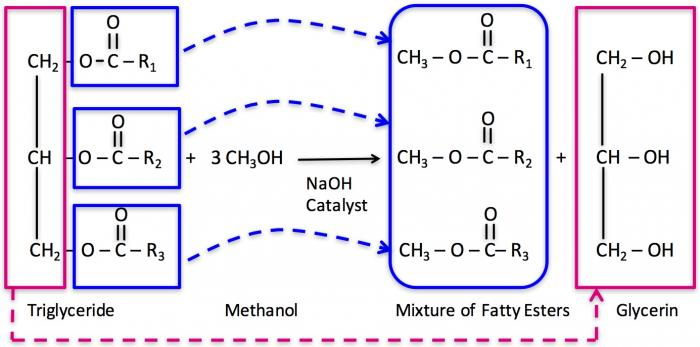
\includegraphics[width=0.8\textwidth]{transesterificacio.jpg}
\end{center}

Aquest procés es realitza generalment afegint un alcohol a l'oli. El metanol (\ch{CH3OH}) és l'alcohol més utilitzat per la seva abundància i baix cost, encara que qualsevol alcohol de cadena curta pot dur a terme la reacció de transesterificació. Aquesta reacció és sovint lenta a causa de la resistència a la desprotonació de l'alcohol, i per això s'afegeix una base forta (com \ch{NaOH}), que té dues funcions: neutralitzar els àcids grassos lliures i desprotonar l'alcohol per formar un anió alcoxi reactiu.

La barreja d'oli vegetal, alcohol i base es remena i es deixa reaccionar. El resultat són dues capes orgàniques separades: una amb els èsters dels àcids grassos i una altra amb glicerina contaminada amb impureses. La capa d'èsters d'àcids grassos es retira i està pràcticament llesta per a l'ús. En algunes estratègies de producció de biodièsel, aquesta capa es renta amb aigua per eliminar impureses solubles en aigua, incloent-hi la base i l'alcohol residuals. L'alcohol també es pot recuperar desti\lgem ant la capa no rentada d'èsters d'àcids grassos. Un cop separades la capa aquosa i la dels èsters d'àcids grassos, aquests últims es sequen i s'emmagatzemen per a ser utilitzats en vehicles dièsel.

El biodièsel presenta diversos avantatges i inconvenients en comparació amb el dièsel derivat del petroli. Un avantatge important és la seva manca de sofre. El biodièsel és essencialment un combustible lliure de sofre, mentre que el dièsel de petroli conté diverses quantitats de sofre. L'absència de sofre en el biodièsel implica que no contribueix significativament a la formació de gasos \ch{SO_x}, responsables de la pluja àcida. A més, estudis han demostrat que el biodièsel pur genera nivells més baixos d'hidrocarburs policíclics aromàtics (PAH), que es consideren cancerígens, així com nivells baixos d'hidrocarburs incombustos, monòxid de carboni (\ch{CO}), diòxid de carboni (\ch{CO2}) i òxids de nitrogen (\ch{NO_x}).

Tanmateix, el biodièsel conté diferents tipus de molècules en comparació amb el dièsel derivat del petroli i, per tant, pot accelerar la degradació de materials orgànics com mànegues i juntes de goma. Alguns dels beneficis del biodièsel també es poden obtenir utilitzant mescles de biodièsel i dièsel de petroli. Hi ha diverses categories estàndard de mescla, i el B-20 (una mescla amb un 20\% de biodièsel) ha demostrat reduir les emissions contaminants en comparació amb el dièsel pur.

Com en el cas de l'etanol, determinar si el biodièsel és realment un benefici energètic requereix una anàlisi completa del cicle de vida. No obstant això, convertir un flux de residus com l'oli vegetal usat en combustible pot ser una avantatge energètica i és un gran projecte per fer-hi recerca.


\section{Tecnologia de Reducció Catalítica Selectiva (SCR)}

Un sistema SCR injecta un producte (Diesel Exhaust Fluid (DEF), conegut comercialment com AdBlue\copyright) en els gasos d'escapament calents, on es descompon en amoníac, que després reacciona a la superfície del catalitzador per produir nitrogen i vapor d'aigua.
L'amoníac (\ch{NH3}) s'utilitza com a agent reductor; no obstant això, a causa de la seva agressivitat i toxicitat, no s'aplica directament, sinó en forma d'una substància innòcua que allibera \ch{NH3} en el corrent de gasos d'escapament. Això permet que el motor funcioni en condicions òptimes, minimitzant així el consum de combustible i, per tant, les emissions de \ch{CO}, així com la descàrrega de tots els contaminants excepte \ch{NO_x}.

Després que els gasos de combustió hagin sortit del motor, primer passen a través d'un catalitzador d'oxidació previ, on els hidrocarburs, el monòxid de carboni i les partícules no cremades s'oxiden tan completament com sigui possible. El \ch{NO} s'oxida parcialment a \ch{NO2}, ja que la reducció posterior es produeix més ràpidament amb una proporció de mescla \ch{NO} : \ch{NO2} de 1:1. A continuació, una bomba, controlada per una unitat de monitoratge, injecta AdBlue des d'un tanc separat en el corrent de gasos d'escapament calents, on es produeix la hidròlisi a \ch{NH3} i \ch{CO2}. En la reducció catalítica selectiva pròpiament dita, l'\ch{NH3} reacciona amb la barreja \ch{NO}/\ch{NO2} per formar nitrogen i aigua (vapor), que constitueixen el 80~\% de la composició natural de l'atmosfera.

AdBlue és una solució aquosa que conté un \qty{32.5}{\percent} d'urea d'alta puresa (per pes) en aigua desionitzada. L'amoníac es genera en fase gasosa mitjançant les següents reaccions\cite{selleri_overview_2021}:

\begin{align}
    \ch{(NH2)2CO(aq)} &\rightarrow \ch{(NH2)2CO(s\ or\ l)} + 6.9 \ch{H2O(g)} && \text{(evaporació de l'aigua)} \\
    \ch{(NH2)2CO(s\ o\ l)} &\rightarrow \ch{NH3(g)} + \ch{HNCO(g)} && \text{(termòlisi de la urea)} \\
    \ch{HNCO(g)} + \ch{H2O(g)} &\rightarrow \ch{NH3(g)} + \ch{CO2(g)} && \text{(hidròlisi de l'àcid isociànic)}
\end{align}

En conjunt, el procés SCR es basa en les següents reaccions globals, que tenen lloc en fase gasosa o adsorbida:

\begin{align}
    4 \ch{NH3} + 4 \ch{NO} + \ch{O2} &\rightarrow 4 \ch{N2} + 6 \ch{H2O} && \text{(SCR estàndard)} \\
    2 \ch{NH3} + \ch{NO} + \ch{NO2} &\rightarrow 2 \ch{N2} + 3 \ch{H2O} && \text{(SCR ràpid)} \\
    8 \ch{NH3} + 6 \ch{NO2} &\rightarrow 7 \ch{N2} + 12 \ch{H2O} && \text{(SCR amb NO2)}
\end{align}

Entre aquestes, la reacció més ràpida és la SCR ràpida, que ocorre quan hi ha una quantitat equimolar de \ch{NO} i \ch{NO2} en els gasos d'escapament. Per aquest motiu, s'ha introduït un catalitzador d'oxidació dièsel (DOC) per assegurar l'oxidació de \ch{NO} a \ch{NO2}. Els DOCs estan guanyant atenció en estudis recents per complir amb regulacions més estrictes, com es veu a la Figura \ref{Fig:ATS}.

\begin{figure}[h!]
    \centering
    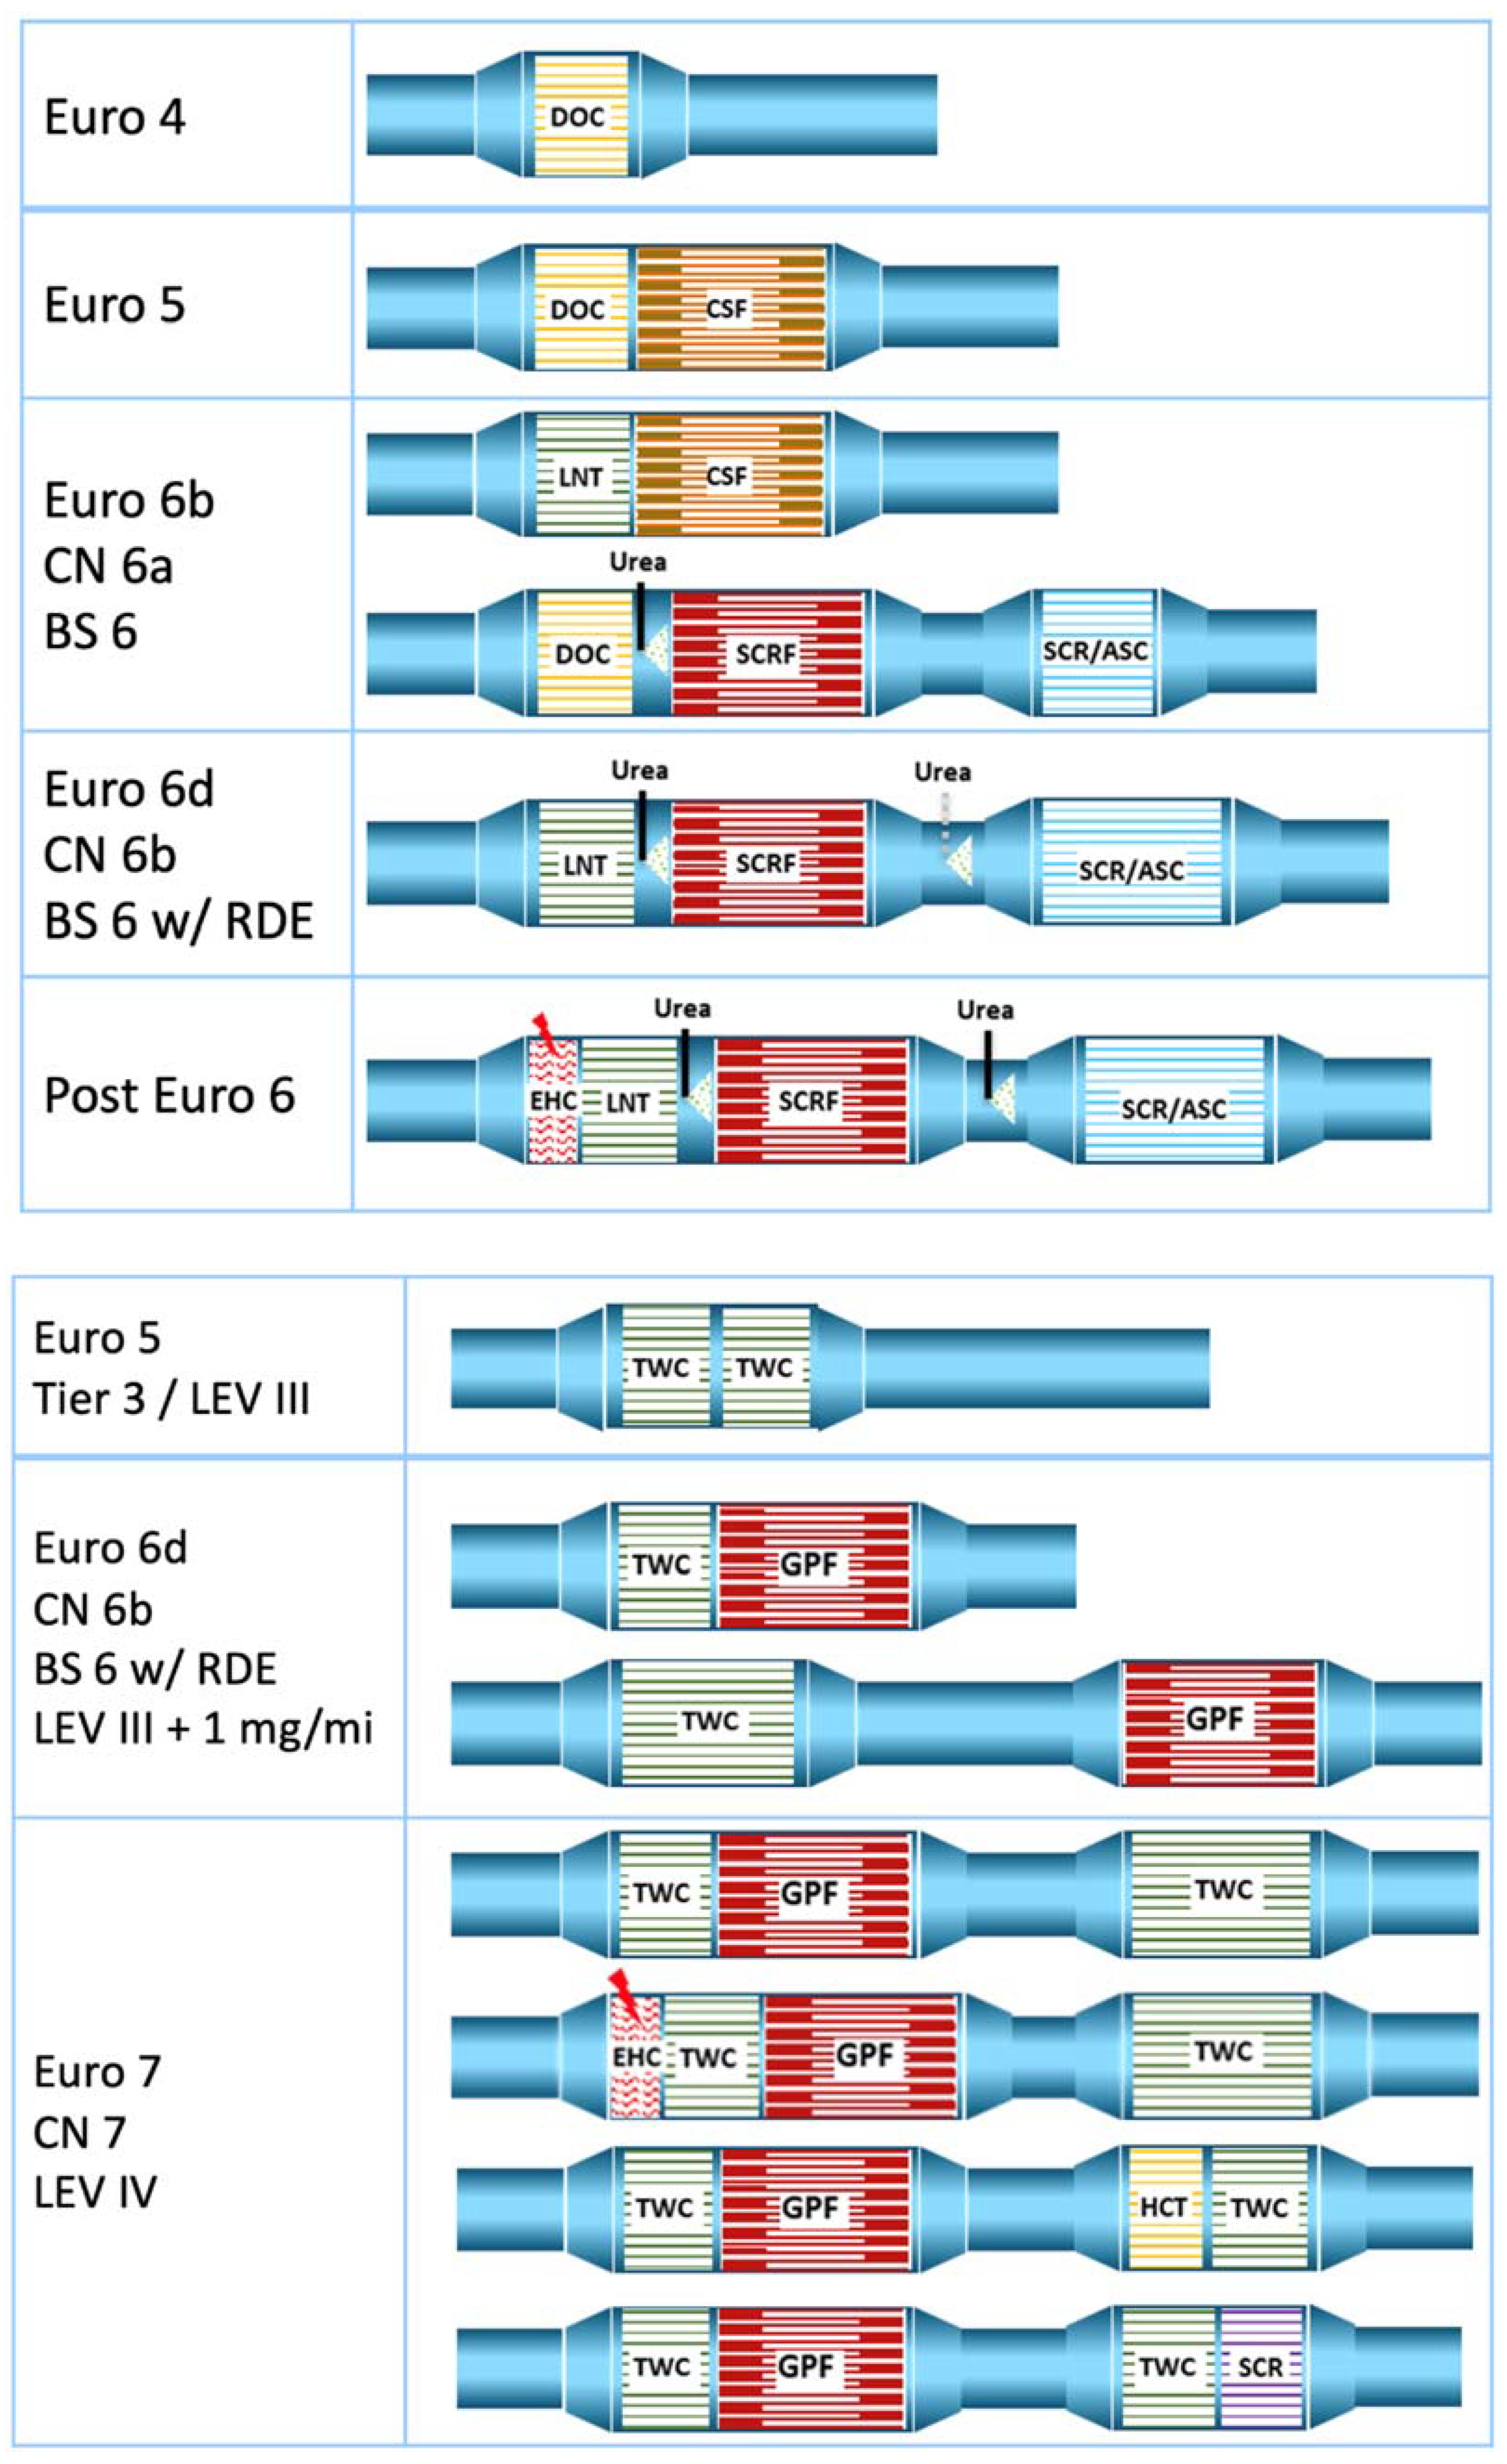
\includegraphics[width=0.7\textwidth]{postexhaustion.png}
    \caption{Evolució de la configuració dels sistemes de postractament (ATS) per a motors Diesel (a dalt) i de benzina (a baix) en vehicles lleugers\cite{selleri_overview_2021}.}
    \label{Fig:ATS}
\end{figure}

A més de les reaccions esmentades, es poden produir reaccions no desitjades, com l'oxidació selectiva de l'amoníac a nitrogen o la seva conversió no selectiva a \ch{NOx}, reduint així l'eficiència del procés: 

\begin{align}
    4 \ch{NH3} + 3 \ch{O2} &\rightarrow 2 \ch{N2} + 6 \ch{H2O} && \text{(oxidació selectiva de l'amoníac)} \\
    4 \ch{NH3} + 5 \ch{O2} &\rightarrow 4 \ch{NO} + 6 \ch{H2O} && \text{(oxidació no selectiva a NO)} \\
    2 \ch{NH3} + 2 \ch{O2} &\rightarrow \ch{N2O} + 2 \ch{H2O} && \text{(oxidació no selectiva a \ch{N2O})}
\end{align}

Aquestes reaccions es tornen rellevants a temperatures altes (superiors a \qty{400}{\degC}) i en absència de \ch{NO2} en l'alimentació. Per contra, una alta presència de \ch{NO2} a baixes temperatures pot conduir a la formació no desitjada de nitrat d'amoni i \ch{N2O}:

\begin{align}
    2 \ch{NH3} + 2 \ch{NO2} &\rightarrow \ch{NH4NO3} + \ch{N2} + \ch{H2O} && \text{(formació de nitrat d'amoni)} \\
    2 \ch{NH3} + 2 \ch{NO2} &\rightarrow \ch{N2O} + \ch{N2} + 3 \ch{H2O} && \text{(formació d'òxid nitrós)}
\end{align}

La formació de nitrat d'amoni és crítica per sota de \qty{180}{\degC}, limitant l'eficàcia del procés SCR a temperatures baixes. No obstant això, aquest compost pot ser reduït per \ch{NO} a \qty{200}{\degC}, generant \ch{NO2} i possibilitant la reacció SCR ràpida, especialment en sistemes catalítics com els Fe-zeolites i \ch{V2O5}-\ch{WO3}/\ch{TiO2}.

Finalment, la presència de sofre en el combustible, combinada amb la funció oxidativa del DOC, pot conduir a la formació de \ch{SO3} i, posteriorment, de sulfats i àcid sulfúric:

\begin{align}
    \ch{SO3} + \ch{H2O} &\rightarrow \ch{H2SO4} && \text{(formació d'àcid sulfúric)} \\
    \ch{NH3} + \ch{SO3} + \ch{H2O} &\rightarrow \ch{(NH4)HSO4} && \text{(formació de bisulfat d'amoni)} \\
    2 \ch{NH3} + \ch{SO3} + \ch{H2O} &\rightarrow \ch{(NH4)2SO4} && \text{(formació de sulfat d'amoni)}
\end{align}

Aquests compostos poden acumular-se al catalitzador, bloquejant-ne els porus i provocant desactivació, tot i que aquest efecte és reversible amb un augment de temperatura. L'àcid sulfúric també pot provocar corrosió en els components del sistema de posttractament i la formació d'aerosols nocius.


Per saber-ne més, consulteu \cite{selleri_overview_2021}.